\chapter{Estratégia de síntese e química verde}\label{ch:g12:synthesis-strategy}

O mesmo analgésico, o ibuprofeno, já foi fabricado de duas maneiras. A
rota mais antiga tem seis etapas, e de cada cem quilogramas de matérias-primas
que ela compra, sessenta viram resíduo. A mais nova tem três etapas, e
aproveita quase todos os \omterm{def:g7:atoms-and-molecules:atom}{átomos} que compra. As duas dão o mesmo pó branco
no comprimido; elas diferem no planejamento. Um químico que planeja uma
\omterm{def:g10:synthesis-yield:synthesis}{síntese} faz quatro perguntas: como ir depressa, como obter muito, como
mexer só na parte certa de uma \omterm{def:g7:atoms-and-molecules:molecule}{molécula}, e como desperdiçar pouco.

\begin{recall}
Uma \omterm{def:g10:synthesis-yield:synthesis}{síntese}: reação, separação, purificação, identificação; o seu
\omterm{def:g10:synthesis-yield:yield}{rendimento} (\cref{ch:g10:synthesis-yield}). As \omterm{def:g12:curly-arrows:curly-arrow}{setas curvas}, a
substituição, a adição, a \omterm{def:g12:curly-arrows:categories}{eliminação} (\cref{ch:g12:curly-arrows}). Um
\omterm{def:g12:catalysis:catalyst}{catalisador} acelera uma reação sem ser consumido (\cref{ch:g12:catalysis}).
Uma \omterm{def:g12:equilibrium:non-total}{reação não total} para em $Q = K$; um excesso de um \omterm{def:g7:chemical-reactions:reactant}{reagente}, ou a
retirada de um produto, a leva mais longe (\cref{ch:g12:equilibrium}).
\end{recall}

\begin{omfigure}
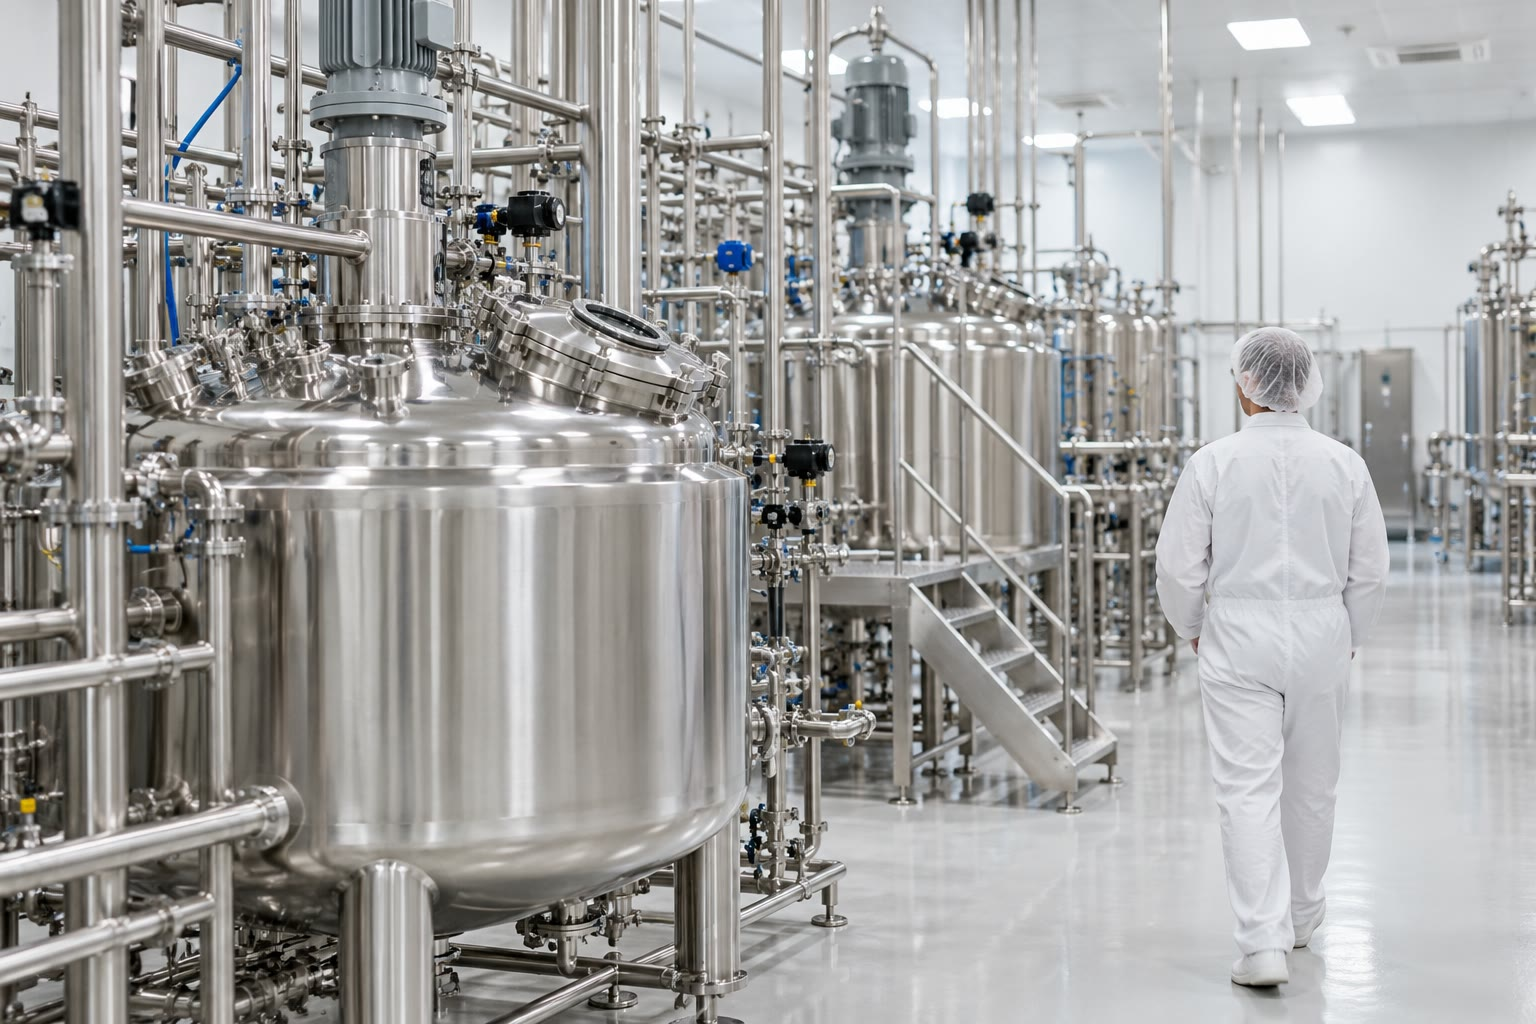
\includegraphics[width=0.48\linewidth]{images/book1/ai/g12-pharma-plant.jpg}

{\small Uma fábrica farmacêutica: os reatores de uma \omterm{def:g10:synthesis-yield:synthesis}{síntese}, ampliados
para toneladas.}
\end{omfigure}

\section{Otimizar uma síntese}

Duas coisas diferentes podem ser melhoradas: a \emph{velocidade}, que
decide quanto tempo a \omterm{def:g10:synthesis-yield:synthesis}{síntese} leva, e o \emph{\omterm{def:g10:synthesis-yield:yield}{rendimento}}, que decide
quanto produto ela dá.

\begin{proposition}[Alavancas sobre a velocidade e o rendimento]\label{prop:g12:synthesis-strategy:levers}
\begin{itemize}
  \item A velocidade aumenta com a temperatura, com as concentrações dos
        \omterm{def:g7:chemical-reactions:reactant}{reagentes} e com um \omterm{def:g12:catalysis:catalyst}{catalisador}.
  \item O \omterm{def:g10:synthesis-yield:yield}{rendimento} final de uma \omterm{def:g10:reaction-progress-table:limiting}{reação total} é fixado pelo \omterm{def:g10:reaction-progress-table:limiting}{reagente
        limitante}; o de uma \omterm{def:g12:equilibrium:non-total}{reação não total} aumenta com um excesso de
        um \omterm{def:g7:chemical-reactions:reactant}{reagente}, ou com a retirada de um produto à medida que ele se
        forma. Um \omterm{def:g12:catalysis:catalyst}{catalisador} não o muda: ele só leva o sistema mais
        depressa ao mesmo \omterm{def:g10:reaction-progress-table:system}{estado final}.
\end{itemize}
\end{proposition}

\begin{proof}
O primeiro ponto reúne os \omterm{def:g12:reaction-rates:kinetic-factor}{fatores cinéticos} dos
\cref{ch:g12:reaction-rates,ch:g12:catalysis}. O segundo decorre de
$Q = K$ no fim de uma \omterm{def:g12:equilibrium:non-total}{reação não total}: acrescentar um \omterm{def:g7:chemical-reactions:reactant}{reagente} ou retirar
um produto torna $Q < K$, e a reação continua no sentido direto.
\end{proof}

\begin{example}[A esterificação com um separador de água]\label{ex:g12:synthesis-strategy:trap}
O ácido etanoico e o etanol, um \omterm{def:g10:the-mole:amount}{mol} de cada, só dão \qty{67}{\percent}
de \omterm{def:g11:functional-groups:carboxylic-acid}{éster} no equilíbrio. Se a \omterm{def:g6:pure-substances-and-mixtures:mixture}{mistura} for aquecida sob refluxo num
\omterm{def:g6:solutions-and-solubility:solute}{solvente} que não se mistura com a água, com um pouco de ácido como
\omterm{def:g12:catalysis:catalyst}{catalisador}, o vapor se condensa num tubo lateral, um \emph{separador de
água}: a água, mais densa, se deposita no fundo e fica ali, enquanto o
\omterm{def:g6:solutions-and-solubility:solute}{solvente} volta para o balão. A água sai da reação à medida que se forma,
$Q$ fica abaixo de $K$, e a esterificação vai quase até o fim. O
aquecimento dá a velocidade, o \omterm{def:g12:catalysis:catalyst}{catalisador} mais velocidade, o separador
o \omterm{def:g10:synthesis-yield:yield}{rendimento}.
\end{example}

\begin{omfigure}
\begin{tikzpicture}[font=\small, scale=0.8]
  \pic[transform shape] at (0,0) {hotplate};
  \pic[transform shape] at (0,0) {rbflask={0.55}{orange!20}};
  % the trap: water at the bottom, solvent above, up to the arm
  \fill[cyan!60!blue!40] (1.0,1.75) arc[start angle=180, end angle=360, radius=0.15] -- (1.3,2.3) -- (1.0,2.3) -- cycle;
  \fill[yellow!35] (1.0,2.3) rectangle (1.3,3.25);
  \draw[om glass] (-0.2,3.0) -- (-0.2,3.75) -- (0.2,3.75) -- (0.2,3.55) -- (1.0,3.55) -- (1.0,4.0);
  \draw[om glass] (0.2,3.0) -- (0.2,3.25) -- (1.0,3.25) -- (1.0,1.75) arc[start angle=180, end angle=360, radius=0.15] -- (1.3,4.0);
  \pic[transform shape] at (1.15,4.0) {condenser};
  \draw[omProp, thick, <-] (1.35,2.0) -- (2.6,1.7) node[right, text=black, align=left] {a água se junta\\ no fundo};
  \draw[omProp, thick, <-] (1.35,2.9) -- (2.6,3.1) node[right, text=black, align=left] {o solvente transborda\\ de volta para o balão};
  \draw[omProp, thick, <-] (-0.6,0.6) -- (-1.7,1.1) node[left, text=black, align=right] {ácido, álcool,\\ catalisador, solvente};
\end{tikzpicture}

{\small Um separador de água num balão aquecido sob refluxo: a água
formada é retirada da reação à medida que se condensa.}
\end{omfigure}

\section{A seletividade}

Uma \omterm{def:g7:atoms-and-molecules:molecule}{molécula} real muitas vezes carrega vários \omterm{def:g11:functional-groups:functional-group}{grupos funcionais}. Um
\omterm{def:g7:chemical-reactions:reactant}{reagente} que ataca todos eles dá uma \omterm{def:g6:pure-substances-and-mixtures:mixture}{mistura}; uma boa \omterm{def:g10:synthesis-yield:synthesis}{síntese} usa um
\omterm{def:g7:chemical-reactions:reactant}{reagente} que só ataca o grupo que deve ser transformado.

\begin{definition}[Reação quimiosseletiva]\label{def:g12:synthesis-strategy:chemoselective}
Uma reação é \emph{quimiosseletiva}\index{reacao quimiosseletiva@reação quimiosseletiva}
quando, numa \omterm{def:g7:atoms-and-molecules:molecule}{molécula} que carrega vários \omterm{def:g11:functional-groups:functional-group}{grupos funcionais}, o seu
\omterm{def:g7:chemical-reactions:reactant}{reagente} transforma um grupo e deixa os outros intactos.
\end{definition}

\begin{example}[Um redutor que escolhe]\label{ex:g12:synthesis-strategy:nabh4}
O boro-hidreto de sódio, \ce{NaBH4}, reduz o grupo carbonila dos
\omterm{def:g11:functional-groups:carbonyl}{aldeídos} e das \omterm{def:g11:functional-groups:carbonyl}{cetonas} a um grupo \omterm{def:g11:functional-groups:alcohol}{álcool}, mas não mexe nos \omterm{def:g11:functional-groups:carboxylic-acid}{ésteres}.
Numa \omterm{def:g7:atoms-and-molecules:molecule}{molécula} que carrega uma \omterm{def:g11:functional-groups:carbonyl}{cetona} e um \omterm{def:g11:functional-groups:carboxylic-acid}{éster}, só a \omterm{def:g11:functional-groups:carbonyl}{cetona} muda:
\[
  \ce{CH3-CO-CH2-CH2-CO-O-CH3}
  \;\xrightarrow{\ \ce{NaBH4}\ }\;
  \ce{CH3-CH(OH)-CH2-CH2-CO-O-CH3} .
\]
Um \omterm{def:g11:redox:oxidant}{redutor} mais forte, o hidreto de lítio e alumínio \ce{LiAlH4},
reduziria os dois grupos: ele não é \omterm{def:g12:synthesis-strategy:chemoselective}{quimiosseletivo} aqui.
\end{example}

\begin{remark}[Vários tipos de seletividade]\label{rem:g12:synthesis-strategy:kinds}
A quimiosseletividade escolhe entre grupos. Uma reação também pode
escolher entre duas posições do mesmo grupo, ou entre dois
\omterm{def:g12:stereochemistry:stereoisomer}{estereoisômeros} do produto, como mostraram as \omterm{def:g12:catalysis:enzyme}{enzimas} do
\cref{ch:g12:catalysis} e as \omterm{def:g7:atoms-and-molecules:molecule}{moléculas} \omterm{def:g12:stereochemistry:chiral}{quirais} do
\cref{ch:g12:stereochemistry}. Cada tipo é estudado nos volumes
universitários.
\end{remark}

\section{Os grupos protetores}

Quando nenhum \omterm{def:g7:chemical-reactions:reactant}{reagente} é seletivo o bastante, o químico esconde o grupo
que não deve reagir, faz a reação e depois descobre o grupo de novo.

\begin{definition}[Grupo protetor]\label{def:g12:synthesis-strategy:protecting-group}
Um \emph{grupo protetor}\index{grupo protetor} é um grupo ligado a um
\omterm{def:g11:functional-groups:functional-group}{grupo funcional} para impedi-lo de reagir durante uma ou mais etapas de
uma \omterm{def:g10:synthesis-yield:synthesis}{síntese}, e retirado depois para devolver o grupo original. As três
operações são a \emph{proteção}, a \emph{reação} e a
\emph{desproteção}.
\end{definition}

\begin{method}[Planejar uma proteção]\label{met:g12:synthesis-strategy:plan}
\begin{enumerate}
  \item Liste os grupos de cada \omterm{def:g7:chemical-reactions:reactant}{reagente}, e a única ligação a formar.
  \item Marque todos os outros grupos que o \omterm{def:g7:chemical-reactions:reactant}{reagente} dessa etapa também
        poderia atacar.
  \item Proteja cada um deles com um grupo que resista às condições da
        reação e que possa ser retirado em condições suaves que
        conservem a nova ligação.
  \item Faça as contas do custo: cada proteção acrescenta duas etapas,
        proteção e desproteção, e diminui o \omterm{def:g10:synthesis-yield:yield}{rendimento} global.
\end{enumerate}
\end{method}

\begin{example}[Fabricar um dipeptídeo, e não quatro]\label{ex:g12:synthesis-strategy:dipeptide}
A glicina, \ce{H2N-CH2-COOH}, e a alanina, \ce{H2N-CH(CH3)-COOH}, carregam
cada uma um grupo \omterm{def:g11:functional-groups:amine}{amina} e um grupo ácido. Uma ligação \omterm{def:g11:functional-groups:amine}{amida} entre o
ácido da glicina e a \omterm{def:g11:functional-groups:amine}{amina} da alanina dá o dipeptídeo Gly--Ala.
\omterm{def:g2:mixing-and-dissolving:mix}{Misturados} diretamente, os dois aminoácidos dão quatro dipeptídeos,
Gly--Ala, Ala--Gly, Gly--Gly e Ala--Ala, numa \omterm{def:g6:pure-substances-and-mixtures:mixture}{mistura} difícil de
separar. O plano:
\begin{enumerate}
  \item proteger a \omterm{def:g11:functional-groups:amine}{amina} da glicina com um grupo escrito \ce{Z}, e o
        ácido da alanina na forma do seu \omterm{def:g11:functional-groups:carboxylic-acid}{éster} metílico;
  \item formar a ligação \omterm{def:g11:functional-groups:amine}{amida}: só sobram livres um grupo ácido e um
        grupo \omterm{def:g11:functional-groups:amine}{amina};
  \item retirar os dois \omterm{def:g12:synthesis-strategy:protecting-group}{grupos protetores}.
\end{enumerate}
\end{example}

\begin{omfigure}
\begin{tikzpicture}[font=\small, node distance=0.55cm,
    box/.style={draw=omDef, rounded corners=2pt, fill=omDef!6, align=center, inner sep=4pt}]
  \node[box] (a) {\ce{H2N-CH2-COOH}\\ \ce{H2N-CH(CH3)-COOH}};
  \node[box, below=of a] (b) {\ce{Z-NH-CH2-COOH}\\ \ce{H2N-CH(CH3)-CO-O-CH3}};
  \node[box, below=of b] (c) {\ce{Z-NH-CH2-CO-NH-CH(CH3)-CO-O-CH3}};
  \node[box, below=of c] (d) {\ce{H2N-CH2-CO-NH-CH(CH3)-COOH}};
  \draw[->, thick, omProp] (a) -- node[right, xshift=3pt, text=black] {1. proteção} (b);
  \draw[->, thick, omProp] (b) -- node[right, xshift=3pt, text=black] {2. reação: ligação amida} (c);
  \draw[->, thick, omProp] (c) -- node[right, xshift=3pt, text=black] {3. desproteção} (d);
  \node[anchor=east, font=\footnotesize, text=black!70] at ([xshift=-6pt]a.west) {glicina, alanina};
  \node[anchor=east, font=\footnotesize, text=black!70] at ([xshift=-6pt]d.west) {Gly--Ala};
\end{tikzpicture}

{\small Proteção, reação, desproteção: a única ligação \omterm{def:g11:functional-groups:amine}{amida} que pode se
formar é a desejada.}
\end{omfigure}

\section{A economia atômica}

Um \omterm{def:g10:synthesis-yield:yield}{rendimento} de \qty{100}{\percent} diz que cada \omterm{def:g7:atoms-and-molecules:molecule}{molécula} do \omterm{def:g10:reaction-progress-table:limiting}{reagente
limitante} virou produto. Ele não diz quantos dos \omterm{def:g7:atoms-and-molecules:atom}{átomos} comprados
acabaram no produto: os outros produtos da equação, por mais puros que
sejam, são resíduos, a menos que alguém possa usá-los.

\begin{definition}[Economia atômica]\label{def:g12:synthesis-strategy:atom-economy}
A \emph{economia atômica}\index{economia atomica@economia atômica} de uma \omterm{def:g10:synthesis-yield:synthesis}{síntese} é a
fração da massa dos \omterm{def:g7:chemical-reactions:reactant}{reagentes}, tomados nas proporções da \omterm{def:g8:balanced-equations:equation}{equação
balanceada}, que acaba no produto desejado.
\end{definition}

\begin{proposition}[A economia atômica a partir da equação]\label{prop:g12:synthesis-strategy:atom-economy}
Para uma \omterm{def:g8:balanced-equations:equation}{equação balanceada} $a_1\,\ce{R1} + a_2\,\ce{R2} + \cdots \rightarrow
p\,\ce{P} + \text{outros produtos}$,
\[
  \text{economia atômica} =
  \frac{p\,M(\ce{P})}{a_1 M(\ce{R1}) + a_2 M(\ce{R2}) + \cdots}
  \times 100\,\% .
\]
\end{proposition}

\begin{proof}
Para $x$ \omterm{def:g10:the-mole:amount}{mols} de reação, a massa de \omterm{def:g7:chemical-reactions:reactant}{reagentes} consumida é
$x\,(a_1 M(\ce{R1}) + \cdots)$ e a massa de produto desejado formada é
$x\,p\,M(\ce{P})$; a sua razão não depende de $x$.
\end{proof}

\begin{method}[Calcular uma economia atômica]\label{met:g12:synthesis-strategy:atom-economy}
\begin{enumerate}
  \item Escreva a \omterm{def:g8:balanced-equations:equation}{equação balanceada}; para uma rota de várias etapas,
        some as etapas de modo que todos os intermediários se cancelem.
  \item Calcule a \omterm{def:g10:the-mole:molar-mass}{massa molar} de cada \omterm{def:g7:chemical-reactions:reactant}{reagente} e do produto desejado.
  \item Aplique a fórmula, com os \omterm{def:g8:balanced-equations:coefficient}{coeficientes estequiométricos}.
  \item O resíduo por quilograma de produto é de
        $(100 - \text{economia atômica})/\text{economia atômica}$ quilogramas.
\end{enumerate}
\end{method}

\begin{example}[Adição contra substituição]\label{ex:g12:synthesis-strategy:compare}
% ledger: aw:C, aw:H, aw:Br, aw:Na, aw:O
O bromoetano a partir do eteno, \ce{C2H4 + HBr -> C2H5Br}: todos os
\omterm{def:g7:atoms-and-molecules:atom}{átomos} acabam no produto, \omterm{def:g12:synthesis-strategy:atom-economy}{economia atômica} $108.9/(28.0 + 80.9) = \qty{100}{\percent}$.
O etanol a partir do bromoetano, \ce{C2H5Br + NaOH -> C2H5OH + NaBr}: a
\omterm{def:g12:synthesis-strategy:atom-economy}{economia atômica} é $46.0/(108.9 + 40.0) = \qty{30.9}{\percent}$; por
quilograma de etanol, \qty{2.2}{kg} de brometo de sódio. Uma adição
sempre tem uma \omterm{def:g12:synthesis-strategy:atom-economy}{economia atômica} de \qty{100}{\percent}; uma substituição
ou uma \omterm{def:g12:curly-arrows:categories}{eliminação} nunca tem.
\end{example}

\begin{omfigure}
\begin{tikzpicture}
\begin{axis}[width=0.8\linewidth, height=5.2cm, ybar, bar width=16pt,
    ymin=0, ymax=112, ylabel={economia atômica (\%)},
    xtick={1,2,3,4,5}, xticklabels={adição, esterificação, ibuprofeno (3 etapas), ibuprofeno (6 etapas), substituição},
    xticklabel style={font=\footnotesize, align=center, text width=2.1cm},
    nodes near coords, nodes near coords style={font=\footnotesize},
    enlarge x limits=0.12, axis lines*=left, ymajorgrids, grid style={black!12}]
  \addplot[fill=omDef!55, draw=omDef] table[x=i, y=AE] {figdata/out/grade-12-synthesis-strategy.dat};
\end{axis}
\end{tikzpicture}

{\small \omterm{def:g12:synthesis-strategy:atom-economy}{Economias atômicas} calculadas a partir das equações: o eteno com
o brometo de hidrogênio, o ácido etanoico com o etanol, as duas rotas do
ibuprofeno, e o bromoetano com o hidróxido de sódio.}
\end{omfigure}

\section{A química verde}

\begin{definition}[Química verde]\label{def:g12:synthesis-strategy:green-chemistry}
A \emph{química verde}\index{quimica verde@química verde} é a concepção de produtos e
de processos químicos que reduzem ou eliminam o uso e a produção de
substâncias perigosas, da escolha das matérias-primas ao destino do
produto depois do uso.
\end{definition}

Doze princípios resumem a abordagem; cada um é uma pergunta a fazer
sobre um processo.
% ledger: green:12
\begin{enumerate}
  \item Prevenir os resíduos em vez de tratá-los.
  \item Maximizar a \omterm{def:g12:synthesis-strategy:atom-economy}{economia atômica}.
  \item Conceber \omterm{def:g10:synthesis-yield:synthesis}{sínteses} menos perigosas.
  \item Conceber produtos químicos e produtos mais seguros.
  \item Usar \omterm{def:g6:solutions-and-solubility:solute}{solventes} e condições de reação mais seguros.
  \item Aumentar a eficiência energética: trabalhar perto da temperatura
        e da pressão ambientes.
  \item Usar matérias-primas renováveis.
  \item Evitar derivados químicos, como os \omterm{def:g12:synthesis-strategy:protecting-group}{grupos protetores}.
  \item Usar \omterm{def:g12:catalysis:catalyst}{catalisadores}, e não \omterm{def:g7:chemical-reactions:reactant}{reagentes} estequiométricos.
  \item Conceber produtos que se degradem depois do uso.
  \item Analisar em tempo real para prevenir a poluição.
  \item Minimizar o potencial de acidentes.
\end{enumerate}

\begin{remark}[Princípios, não leis]\label{rem:g12:synthesis-strategy:principles}
Os princípios muitas vezes puxam em sentidos opostos: um \omterm{def:g12:synthesis-strategy:protecting-group}{grupo protetor}
desrespeita o princípio 8, mas pode salvar uma \omterm{def:g10:synthesis-yield:synthesis}{síntese} inteira; um
\omterm{def:g12:catalysis:catalyst}{catalisador} que economiza energia pode conter um \omterm{def:g9:periodic-table-first-look:metal}{metal} raro. Julgar um
processo é pesar os princípios, com números sempre que possível:
\omterm{def:g12:synthesis-strategy:atom-economy}{economia atômica}, \omterm{def:g10:synthesis-yield:yield}{rendimento}, massa de resíduos, energia.
\end{remark}

\begin{history}[A química verde, 1998]
% ledger: green:book-1998, ibu:bhc-commercial
Em 1998, os químicos Paul Anastas e John Warner publicaram um livro,
\emph{Green Chemistry: Theory and Practice}, que expôs os doze
princípios. Um ano antes, um prêmio do governo para \omterm{def:g10:synthesis-yield:synthesis}{sínteses} mais
verdes tinha ido para a rota de três etapas do ibuprofeno, usada em
escala industrial desde 1992. Desde então, os princípios são ensinados
aos químicos como parte do seu ofício.
\end{history}

\begin{example}[Duas rotas para o ibuprofeno]\label{ex:g12:synthesis-strategy:ibuprofen}
% ledger: ibu:boots-steps, ibu:bhc-steps, ibu:boots-ae, ibu:bhc-ae, ibu:bhc-ae-recovered
O ibuprofeno, \ce{C13H18O2}, é fabricado a partir do hidrocarboneto
\ce{C10H14} (isobutilbenzeno). A rota mais antiga usa seis etapas e, em
cada uma, uma quantidade completa de \omterm{def:g7:chemical-reactions:reactant}{reagente}; somados, os seus
\omterm{def:g7:chemical-reactions:reactant}{reagentes} têm uma soma de \omterm{def:g10:the-mole:molar-mass}{massas molares} de \qty{514.5}{g/mol}, para
\qty{206.0}{g/mol} de ibuprofeno: \omterm{def:g12:synthesis-strategy:atom-economy}{economia atômica} de
\qty{40}{\percent}. A rota mais nova usa três etapas, duas delas
catalisadas, e a equação global
\[
  \ce{C10H14 + C4H6O3 + H2 + CO -> C13H18O2 + C2H4O2}
\]
dá $206.0/266.0 = \qty{77}{\percent}$. O seu subproduto, o ácido
etanoico, é recuperado e usado: contado como produto, a \omterm{def:g12:synthesis-strategy:atom-economy}{economia atômica}
passa de \qty{99}{\percent}.
\end{example}

\begin{omfigure}
\chemfig{[:30]*6(-=(-[:90](-[:150])-[:30](=[:90]O)-[:-30]OH)-=-(-[:-90]-[:-150](-[:150])-[:-90])=)}

\medskip
\begin{tikzpicture}[font=\scriptsize,
    st/.style={draw=omDef, rounded corners=2pt, fill=omDef!6, minimum height=0.8cm, text width=1.15cm, align=center, inner sep=2pt}]
  \foreach \i/\t in {1/acilação, 2/+ 2 carbonos, 3/aldeído, 4/oxima, 5/nitrila, 6/ácido}
    \node[st] (o\i) at (1.7*\i,0) {\t};
  \foreach \i/\j in {1/2,2/3,3/4,4/5,5/6} \draw[->, thick] (o\i) -- (o\j);
  \node[anchor=east, align=right, font=\footnotesize] at ([xshift=-4pt]o1.west) {6 etapas\\ \textbf{40 \%}};
  \foreach \i/\t in {1/acilação, 2/adiciona \ce{H2}, 3/adiciona \ce{CO}}
    \node[st, fill=omProp!8, draw=omProp] (n\i) at (1.7*\i,-1.4) {\t\\ (catálise)};
  \foreach \i/\j in {1/2,2/3} \draw[->, thick] (n\i) -- (n\j);
  \node[anchor=east, align=right, font=\footnotesize] at ([xshift=-4pt]n1.west) {3 etapas\\ \textbf{77 \%}};
  \node[anchor=west, align=left, font=\footnotesize] at ([xshift=6pt]n3.east) {subproduto: ácido etanoico, recuperado;\\ contado como produto: mais de 99 \%};
\end{tikzpicture}

{\small O ibuprofeno (em cima) e as suas duas rotas industriais: a mais
antiga, com seis etapas, e a mais nova, com três etapas catalisadas,
com as suas \omterm{def:g12:synthesis-strategy:atom-economy}{economias atômicas}.}
\end{omfigure}

\begin{example}[Solventes mais verdes]\label{ex:g12:synthesis-strategy:solvents}
% ledger: crit:CO2-T, crit:CO2-p
Muitas reações e \omterm{def:g10:chemical-species:extraction}{extrações} usam \omterm{def:g6:solutions-and-solubility:solute}{solventes} orgânicos tóxicos,
inflamáveis ou voláteis. A água é o mais seguro de todos os \omterm{def:g6:solutions-and-solubility:solute}{solventes},
quando os \omterm{def:g7:chemical-reactions:reactant}{reagentes} se dissolvem nela. O dióxido de carbono vira outro:
acima de \qty{31}{\celsius} e \qty{73.8}{bar}, ele é um \emph{fluido
supercrítico}, nem líquido nem gás, que dissolve muitas \omterm{def:g7:atoms-and-molecules:molecule}{moléculas}
orgânicas. Ele extrai, por exemplo, a cafeína dos grãos de café; quando
a pressão é liberada, ele simplesmente volta a ser gás e não deixa
nenhum resíduo no produto.
\end{example}

\begin{omfigure}
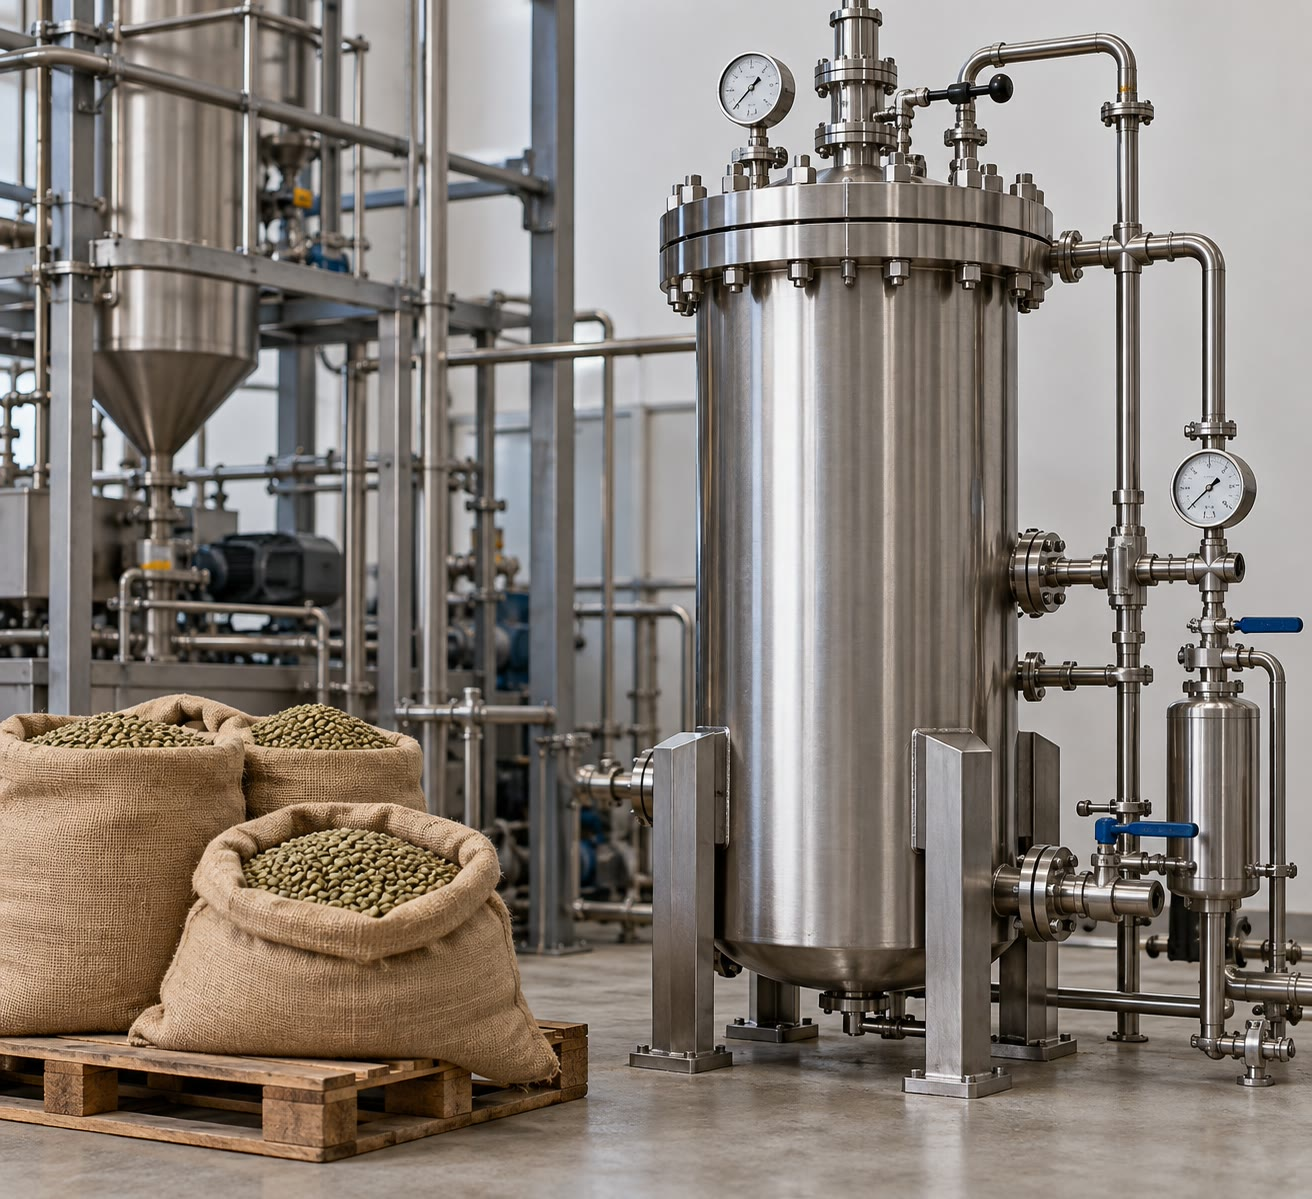
\includegraphics[width=0.45\linewidth,height=6cm,keepaspectratio]{images/book1/ai/g12-scco2-vessel.jpg}

{\small Um vaso de \omterm{def:g10:chemical-species:extraction}{extração} de alta pressão, em que o dióxido de carbono
supercrítico substitui um \omterm{def:g6:solutions-and-solubility:solute}{solvente} orgânico.}
\end{omfigure}

\section{Exercícios}

\begin{exercise}[$\star$]\label{exo:g12:synthesis-strategy:1}
O etanol pode ser fabricado por hidratação do eteno,
\ce{C2H4 + H2O -> C2H5OH}, ou por fermentação da glicose,
\ce{C6H12O6 -> 2C2H5OH + 2CO2}. Calcule a \omterm{def:g12:synthesis-strategy:atom-economy}{economia atômica} de cada uma.
\end{exercise}

\begin{exercise}[$\star$]\label{exo:g12:synthesis-strategy:2}
No esquema do dipeptídeo deste capítulo, diga em que etapa cada \omterm{def:g12:synthesis-strategy:protecting-group}{grupo
protetor} é colocado, e em que etapa ele é retirado.
\end{exercise}

\begin{exercise}[$\star$]\label{exo:g12:synthesis-strategy:3}
Uma fábrica substitui um \omterm{def:g6:solutions-and-solubility:solute}{solvente} clorado por água numa das suas
reações. Que princípio da \omterm{def:g12:synthesis-strategy:green-chemistry}{química verde} ela aplica?
\end{exercise}

\begin{exercise}[$\star$]\label{exo:g12:synthesis-strategy:4}
Por que um excesso de etanol aumenta o \omterm{def:g10:synthesis-yield:yield}{rendimento} de uma esterificação,
e um \omterm{def:g12:catalysis:catalyst}{catalisador} não?
\end{exercise}

\begin{exercise}[$\star$]\label{exo:g12:synthesis-strategy:5}
O boro-hidreto de sódio reduz os \omterm{def:g11:functional-groups:carbonyl}{aldeídos} e as \omterm{def:g11:functional-groups:carbonyl}{cetonas}, não os \omterm{def:g11:functional-groups:carboxylic-acid}{ésteres}.
A sua reação com o 4-oxopentanoato de metila (uma \omterm{def:g11:functional-groups:carbonyl}{cetona} e um \omterm{def:g11:functional-groups:carboxylic-acid}{éster}) é
\omterm{def:g12:synthesis-strategy:chemoselective}{quimiosseletiva}? Que grupo muda?
\end{exercise}

\begin{exercise}[$\star\star$]\label{exo:g12:synthesis-strategy:6}
Um \omterm{def:g10:the-mole:amount}{mol} de ácido etanoico e um de etanol dão \qty{0.67}{mol} de \omterm{def:g11:functional-groups:carboxylic-acid}{éster} no
equilíbrio. Proponha duas maneiras de aumentar essa quantidade, e uma
maneira de chegar a ela mais depressa.
\end{exercise}

\begin{exercise}[$\star\star$]\label{exo:g12:synthesis-strategy:7}
O 4-oxopentanoato de metila, \ce{CH3-CO-CH2-CH2-CO-O-CH3}, é tratado uma
vez com boro-hidreto de sódio, e outra vez com um excesso de hidreto de
lítio e alumínio, que reduz o \omterm{def:g11:functional-groups:carboxylic-acid}{éster} a dois \omterm{def:g11:functional-groups:alcohol}{álcoois}. Escreva cada
produto.
\end{exercise}

\begin{exercise}[$\star\star$]\label{exo:g12:synthesis-strategy:8}
No gráfico de barras das \omterm{def:g12:synthesis-strategy:atom-economy}{economias atômicas}, que reações conservam mais
de três quartos dos \omterm{def:g7:atoms-and-molecules:atom}{átomos}? Por que fator a rota de três etapas do
ibuprofeno é melhor que a de seis?
\end{exercise}

\begin{exercise}[$\star\star$]\label{exo:g12:synthesis-strategy:9}
A aspirina é fabricada por \ce{C7H6O3 + C4H6O3 -> C9H8O4 + C2H4O2}.
Calcule a sua \omterm{def:g12:synthesis-strategy:atom-economy}{economia atômica} e a massa de subproduto por quilograma de
aspirina.
\end{exercise}

\begin{exercise}[$\star\star$]\label{exo:g12:synthesis-strategy:10}
Por que uma \omterm{def:g10:synthesis-yield:synthesis}{síntese} é aquecida sob refluxo e não num balão aberto? Qual
dos dois, a velocidade ou o \omterm{def:g10:synthesis-yield:yield}{rendimento}, o aquecimento melhora?
\end{exercise}

\begin{exercise}[$\star\star$]\label{exo:g12:synthesis-strategy:11}
Na figura das duas rotas do ibuprofeno, conte as etapas e diga que
princípios da \omterm{def:g12:synthesis-strategy:green-chemistry}{química verde} a rota mais nova aplica. Dê três.
\end{exercise}

\begin{exercise}[$\star\star\star$]\label{exo:g12:synthesis-strategy:12}
Uma \omterm{def:g10:synthesis-yield:synthesis}{síntese} de três etapas tem \omterm{def:g10:synthesis-yield:yield}{rendimentos} de \qty{80}{\percent},
\qty{70}{\percent} e \qty{90}{\percent}. Calcule o \omterm{def:g10:synthesis-yield:yield}{rendimento} global.
Que quantidade de \omterm{def:g5:raw-materials-and-recycling:raw-material}{matéria-prima} é necessária para obter \qty{0.10}{mol}
de produto final, sabendo que um \omterm{def:g10:the-mole:amount}{mol} de \omterm{def:g5:raw-materials-and-recycling:raw-material}{matéria-prima} dá no máximo um
\omterm{def:g10:the-mole:amount}{mol} de produto?
\end{exercise}

\begin{exercise}[$\star\star\star$]\label{exo:g12:synthesis-strategy:13}
Planeje a \omterm{def:g10:synthesis-yield:synthesis}{síntese} do dipeptídeo Ala--Gly (o ácido da alanina ligado à
\omterm{def:g11:functional-groups:amine}{amina} da glicina): que grupos você protege, e quantas etapas o plano
tem?
\end{exercise}

\begin{exercise}[$\star\star\star$]\label{exo:g12:synthesis-strategy:14}
Uma empresa chama o seu processo de ``verde'' porque ele usa um
\omterm{def:g12:catalysis:catalyst}{catalisador}. O processo funciona a \qty{250}{\celsius} em benzeno, um
\omterm{def:g6:solutions-and-solubility:solute}{solvente} tóxico, e a sua \omterm{def:g12:synthesis-strategy:atom-economy}{economia atômica} é de \qty{35}{\percent}.
Julgue a afirmação, princípio por princípio.
\end{exercise}

\begin{exercise}[$\star\star\star$]\label{exo:g12:synthesis-strategy:15}
A cafeína é extraída dos grãos de café ou com diclorometano, um \omterm{def:g6:solutions-and-solubility:solute}{solvente}
clorado volátil, ou com dióxido de carbono supercrítico a cerca de
\qty{40}{\celsius} e \qty{100}{bar}. Explique por que o segundo é
supercrítico, por que ele precisa de um vaso resistente, e dê duas
vantagens que ele tem sobre o primeiro.
\end{exercise}

\section{Problema: duas rotas para o ibuprofeno}

\begin{problem}[{Problema de fim de semana --- quanto resíduo a rota de três
etapas evita por tonelada de ibuprofeno?}]
\label{pb:g12:synthesis-strategy:1}
% ledger: ibu:boots-ae, ibu:bhc-ae, ibu:boots-steps, ibu:bhc-steps, aw:C, aw:H, aw:O, aw:N, aw:Cl, aw:Na
A rota mais antiga do ibuprofeno \ce{C13H18O2} tem seis etapas. Somados,
os seus \omterm{def:g7:chemical-reactions:reactant}{reagentes} são \ce{C10H14}, \ce{C4H6O3}, \ce{C4H7ClO2},
\ce{C2H5ONa}, um ácido contado como \ce{H3O}, \ce{NH3O} e dois
\ce{H2O}. A rota mais nova tem três etapas:
\[
  \ce{C10H14 + C4H6O3 + H2 + CO -> C13H18O2 + C2H4O2} .
\]

\medskip
\noindent\textbf{Parte I --- As equações.}
\begin{enumerate}
  \item Verifique que a equação da rota mais nova está balanceada em
        carbono, hidrogênio e oxigênio.
  \item Dê o nome do subproduto da rota mais nova.
  \item Na rota mais antiga, que elementos dos \omterm{def:g7:chemical-reactions:reactant}{reagentes} acabam
        inteiramente nos resíduos?
  \item Qual das duas rotas usa \omterm{def:g12:catalysis:catalyst}{catalisadores}? Que princípio isso
        aplica?
\end{enumerate}

\medskip
\noindent\textbf{Parte II --- As \omterm{def:g12:synthesis-strategy:atom-economy}{economias atômicas}.}
\begin{enumerate}[resume]
  \item Calcule a \omterm{def:g10:the-mole:molar-mass}{massa molar} do ibuprofeno.
  \item Calcule a soma das \omterm{def:g10:the-mole:molar-mass}{massas molares} dos \omterm{def:g7:chemical-reactions:reactant}{reagentes} da rota mais
        antiga.
  \item Deduza a sua \omterm{def:g12:synthesis-strategy:atom-economy}{economia atômica}.
  \item Calcule a soma das \omterm{def:g10:the-mole:molar-mass}{massas molares} dos \omterm{def:g7:chemical-reactions:reactant}{reagentes} da rota mais
        nova.
  \item Deduza a sua \omterm{def:g12:synthesis-strategy:atom-economy}{economia atômica}.
  \item Quanto ela passa a ser se o ácido etanoico for contado como
        produto?
\end{enumerate}

\medskip
\noindent\textbf{Parte III --- Os resíduos por tonelada.}
\begin{enumerate}[resume]
  \item Para a rota mais antiga, com \omterm{def:g10:synthesis-yield:yield}{rendimento} de \qty{100}{\percent},
        que massa de \omterm{def:g7:chemical-reactions:reactant}{reagentes} é comprada por tonelada de ibuprofeno?
  \item Que massa de resíduos ela dá por tonelada?
  \item A mesma pergunta para a rota mais nova: massa de \omterm{def:g7:chemical-reactions:reactant}{reagentes} por
        tonelada.
  \item A massa de ácido etanoico por tonelada.
  \item Que massa de resíduos por tonelada é evitada se o ácido
        etanoico for contado como resíduo?
\end{enumerate}

\medskip
\noindent\textbf{Parte IV --- Os \omterm{def:g10:synthesis-yield:yield}{rendimentos} e o mundo real.}
\begin{enumerate}[resume]
  \item Suponha que cada etapa tenha um \omterm{def:g10:synthesis-yield:yield}{rendimento} de
        \qty{90}{\percent}. Calcule o \omterm{def:g10:synthesis-yield:yield}{rendimento} global da rota mais
        antiga.
  \item O mesmo para a rota mais nova.
  \item Dê mais uma razão pela qual menos etapas significam menos
        resíduos, além da equação.
  \item Na prática, o ácido etanoico é recuperado e usado. Que massa de
        resíduos por tonelada a rota mais nova dá então, com \omterm{def:g10:synthesis-yield:yield}{rendimento}
        de \qty{100}{\percent}?
  \item Dê a resposta final: quanto resíduo a rota de três etapas evita
        por tonelada de ibuprofeno?
\end{enumerate}
\end{problem}
